% Template LaTeX para Informes de Proyectos de Grado de Computación
% InCo, Facultad de Ingeniería, Universidad de la República
% 06/2023

\documentclass{prgrado}

\usepackage[top=2cm, bottom=4cm, left=3cm, right=3cm]{geometry}
\usepackage{caption}
\usepackage{xcolor}
\usepackage{wrapfig}


%%%%%%%%%%%%%%%%%%%%%%%%%%%%%%%%%%%%%%%%%%%%%%%%%%%%%%%%%%%%%%%%%%%%%%%%%%%%%%%%%%%%%%%%%%%%%%%%
% Datos del Proyecto:
%%%%%%%%%%%%%%%%%%%%%%%%%%%%%%%%%%%%%%%%%%%%%%%%%%%%%%%%%%%%%%%%%%%%%%%%%%%%%%%%%%%%%%%%%%%%%%%%

% título del proyecto (debe escribirse en minúscula, con excepción de la
% letra inicial de la primera palabra y nombres propios)
\title{Título que va a poner a su proyecto de grado}                   

% autores
\author{Aguses y Stefa}  

% fecha de la defensa
\date{\today}                                 

% supervisor
\supervisor{Nombre Supervisor}                

% cosupervisor (comentar si no tiene)
\cosupervisor{Nombre Co-Supervisor}

% licencia creative commons del documento
% opciones: by, by-sa, by-nd, by-nc, by-nc-sa y by-nc-nd
% opción por defecto: by-nc-nd versión 4.0
\cclicense{by}{4.0}

%%%%%%%%%%%%%%%%%%%%%%%%%%%%%%%%%%%%%%%%%%%%%%%%%%%%%%%%%%%%%%%%%%%%%%%%%%%%%%%%%%%%%%%%%%%%%%%%


%links con colores 
\hypersetup{
  colorlinks   = true,
  urlcolor     = blue,
  linkcolor    = blue,
  citecolor    = red
}


\begin{document}

%%%%%%%%%%%%%%%%%%%%%%%%%%%%%%%%%%%%%%%%%%%%%%%%%%%%%%%%%%%%%%%%%%%%%%%%%%%%%%%%%%%%%%%%%%%%%%%%
% Parte inicial
%%%%%%%%%%%%%%%%%%%%%%%%%%%%%%%%%%%%%%%%%%%%%%%%%%%%%%%%%%%%%%%%%%%%%%%%%%%%%%%%%%%%%%%%%%%%%%%%

\frontmatter % numeración en romanos, capitulos sin numerar

% carátula
\maketitle


%%%%%%%%%%%%%%%%%%%%%%%%%%%%%%%%%%%%%%%%%%%%%%%%%%%%%%%%%%%%%%%%%%%%%%%%%%%%%%%%%%%%%%%%%%%%%%%%

% agradecimientos
\chapter*{Agradecimientos}

Agradecer, siempre es bueno agradecer.



%%%%%%%%%%%%%%%%%%%%%%%%%%%%%%%%%%%%%%%%%%%%%%%%%%%%%%%%%%%%%%%%%%%%%%%%%%%%%%%%%%%%%%%%%%%%%%%%

% resumen
\chapter*{Resumen}

El resumen (200-500 palabras) debe dar una idea completa de todo el
proyecto, mencionando claramente los formalismos, técnicas, herramientas y lenguajes
utilizados. No debe limitarse a describir el problema abordado, sino que debe describir
la solución del problema, con una evaluación de la misma. No debe incluir referencias
bibliográficas ni referencias a otras partes del informe. Tampoco debe utilizar
acrónimos sin explicar su significado.


\hfill \break
\keywords{Template, Proyectos de Grado, Computación}

%%%%%%%%%%%%%%%%%%%%%%%%%%%%%%%%%%%%%%%%%%%%%%%%%%%%%%%%%%%%%%%%%%%%%%%%%%%%%%%%%%%%%%%%%%%%%%%%

% índice
\tableofcontents
\newpage


%%%%%%%%%%%%%%%%%%%%%%%%%%%%%%%%%%%%%%%%%%%%%%%%%%%%%%%%%%%%%%%%%%%%%%%%%%%%%%%%%%%%%%%%%%%%%%%%
% Parte central
%%%%%%%%%%%%%%%%%%%%%%%%%%%%%%%%%%%%%%%%%%%%%%%%%%%%%%%%%%%%%%%%%%%%%%%%%%%%%%%%%%%%%%%%%%%%%%%%

\mainmatter %numeración en arábicos, numerar capítulos 

% introducción
\chapter{Introducción}

La capacidad de simular y predecir comportamientos es una cualidad altamente valorada en el campo de la ingeniería. Comprender un concepto a tal nivel que se puedan realizar simulaciones desbloquea un gran potencial tanto para fines analíticos y didácticos como para la reducción de costos operativos y de desarrollo. 


En el ámbito audiovisual, la motivación para realizar simulaciones sonoras es diversa. En la industria del cine y los videojuegos, por ejemplo, estas simulaciones permiten crear ambientes sonoros más envolventes y realistas, enriqueciendo significativamente la experiencia del usuario. En el campo de la arquitectura, facilitan a los diseñadores el entendimiento de cómo se propaga el sonido en espacios cerrados, aspecto crucial para el diseño de teatros, salas de conciertos y otros espacios acústicamente sensibles. Además, en la planificación urbana, esta tecnología podría predecir y mitigar la contaminación acústica en las ciudades, mejorando así la calidad de vida de los residentes.


Para simular este fenómeno, se puede recurrir a una analogía con la luz, otro fenómeno físico común cuyas técnicas de simulación están bien establecidas y popularizadas. Una de estas técnicas es el trazado de rayos, comúnmente aplicada en computación gráfica para simular la interacción de los rayos de luz con un entorno y así generar imágenes realistas. Esta técnica ha experimentado avances significativos en las últimas décadas, gracias al progreso en computación que caracteriza a la era actual. Por un lado, la luz y el sonido comparten algunas características comunes, como emanar de una fuente, propagarse en forma de ondas e interactuar con objetos, lo cual indica suficientes paralelismos para poder asumir que el trazado de rayos puede ser aplicado para realizar simulaciones acústicas. Sin embargo, presentan diferencias extremadamente significativas en varios aspectos, como la longitud de onda y la velocidad, entre otros. Estas diferencias implican que la aplicación del trazado de rayos en sonido no es directamente trasladable desde su uso en la luz, sino que debe ser ajustado correspondientemente.


En el ámbito del trazado de rayos, la industria del entretenimiento, especialmente los sectores de videojuegos y efectos visuales, ha sido un motor fundamental en el avance de las técnicas de trazado de rayos. Además, han estimulado el desarrollo de herramientas tecnológicas avanzadas, como las tarjetas gráficas, también conocidas como unidades de procesamiento gráfico (GPU, por sus siglas en inglés). Estas GPUs no solo destacan por su gran potencia, sino que también son suficientemente accesibles para un amplio espectro de usuarios. La accesibilidad de estas tecnologías ha incentivado a los competidores en el mercado a promover su uso en la programación abierta y habilitar a sus usuarios poder utilizar su poder computacional para un fin deseado, por ejemplo, la elaboración de un renderer acústico utilizando trazado de ratos.

%%%%%%%%%%%%%%%%%%%%%%%%%%%%%%%%%%%%%%%%%%%%%%%%%%%%%%%%%%%%%%%%%%%%%%%%%%%%%%%%%%%%%%%%%%%%%%%%

% antecedentes
\chapter{Revisión de antecedentes} 

\section{Fundamentos del sonido}

En el marco del proyecto, la comprensión detallada de los fundamentos del sonido adquiere una importancia crítica, tanto como un pilar teórico sino también por su aplicabilidad directa en las soluciones tecnológicas desarrolladas.

\subsection{La onda de sonido}

\colorbox{yellow}{El sonido se define como .... TODO, a continuación esta lo viejo. El sonido es un fenómeno físico resultante de una cadena de efectos. Partiendo de una fuente que genera vibraciones de pequeña amplitud, estas fluctuaciones de presión se pueden propagar a través de un medio elástico, como el aire, hasta llegar a un receptor, como el oído en los seres vivos \cite{Moser}.}

Tales vibraciones se conducen fácilmente en gases, líquidos y sólidos como el aire, el agua, el acero, etc., que son todos medios elásticos. Si una partícula en uno de estos medios se desplaza de su posición original, las fuerzas elásticas tienden a restaurarla a su posición inicial. Y debido a la inercia de la partícula, ésta sobrepasa la posición de reposo, lo que activa las fuerzas elásticas en la dirección opuesta, y así sucesivamente (Figura~\ref{fig:vibracion}). Por esta razón, la elasticidad y la inercia son dos características que todos los medios deben poseer para ser capaces de conducir el sonido.

\begin{figure}[h!]
    \centering
    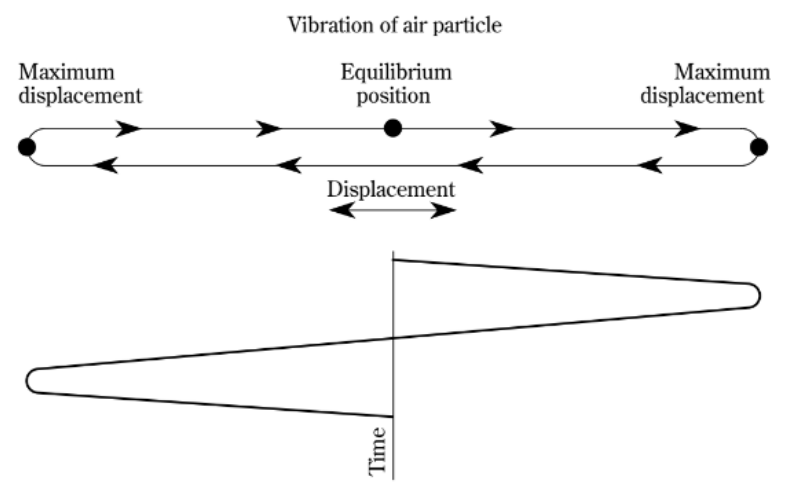
\includegraphics[width=0.7\textwidth]{figs/vibration-of-air-particle.png}
    \captionsetup{justification=centering}
    \caption{Posición en el tiempo de una partícula de aire bajo los efectos de fuerzas elásticas. Extraído de \cite{Everest}}
    \label{fig:vibracion}
\end{figure}

El movimiento previamente descrito en las partículas de un medio constituye la onda sonora. Dicha onda genera la compresión y rarefacción (o escasez) de dichas partículas, (Figura ~\ref{fig:presion})

\begin{figure}[h!]
    \centering
    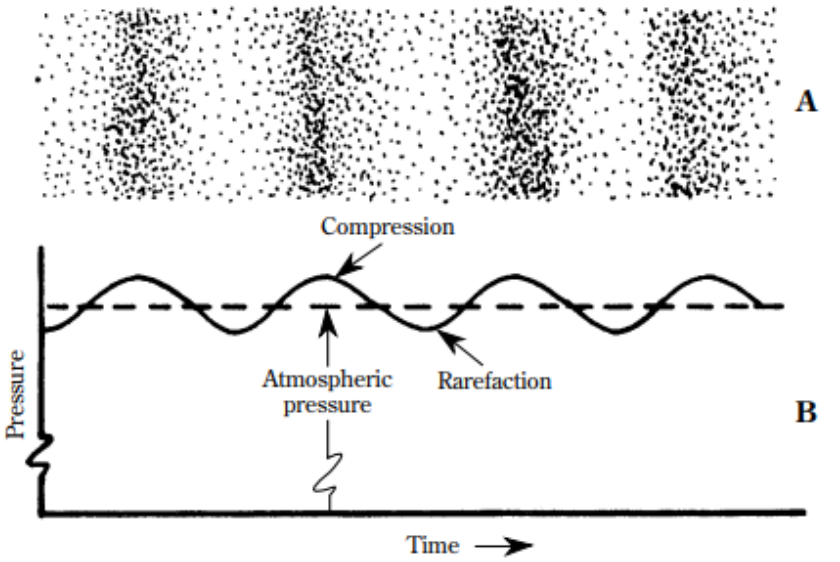
\includegraphics[width=0.6\textwidth]{figs/particle-pressure.png}
    \captionsetup{justification=centering}
    \caption{(A) Ilustración de un grupo de partículas comprimidas y enrarecidas debido a la transmisión del sonido. (B) Variaciones en la presión causadas por una onda de sonido con respecto a la presión atmosférica. Extraído de \cite{Everest}}
    \label{fig:presion}
\end{figure}

La intensidad acústica de un sonido, o volumen, es proporcional al cuadrado de la presión sonora efectiva, la cual es medida en Pascales (Pa). Viéndolo desde una perspectiva matemática, esta presión se representa con la amplitud de la onda, es decir, la diferencia del valor de la presión entre los “valles” y las “crestas”.

Además, la onda sonora exhibe otra propiedad fundamental: su frecuencia, definida como el número de ciclos completos por unidad de tiempo, la cual determina el tono del sonido y es medida en Hertz (Hz).

Finalmente, la longitud de onda representa la distancia en el espacio que se desplaza una onda en el tiempo que esta demora en realizar un ciclo. Dado este valor, es posible calcular la velocidad del sonido\footnote{En la atmósfera terrestre la velocidad del sonido es de 343.2 m/s a 20 °C de temperatura}.

\subsection{Nivel de sonido}

Nuestra percepción del sonido no se relaciona linealmente con los atributos físicos del sonido. Más precisamente, el oído humano percibe cambios en el nivel sonoro de forma logarítmica.

El decibel (dB) es una unidad logarítmica usada para medir la intensidad de un sonido. Cuantifica el nivel sonoro al comparar la presión de dicho sonido con la presión de un sonido referencia (denominado $P_0$) con una presión de 20µPa (micropascales) en el aire, valor que representa la diferencia de presiones entre el momento de compresión y rarefacción de las partículas (es decir, el valle y la cresta de la onda). Este valor aproxima a la mínima presión percibible por un humano con excelentes habilidades auditivas.

La fórmula para el nivel en decibeles de un sonido con una determinada presión $P_1$ es definida de la siguiente forma

\begin{equation}
L = 20 * log_{10}(P_1/P_0)
\end{equation}

Se puede apreciar con esta formula que el nivel sonoro de un sonido con una presión que sea igual al
valor base corresponde a 0 dB.

\subsection{Interacción del sonido con el ambiente}

Mientras las ondas de sonido se propagan, estas interactúan con el ambiente de formas complejas y variadas, dando lugar a distintos fenómenos como la reflexión, absorción, transmisión, refracción y difracción de la onda. En esta sección se procederá a explicar cada fenómeno mencionado.

Cuando una onda de sonido encuentra una superficie u objeto que se consideran “grandes” en comparación a su longitud de onda, la onda de sonido sufre una \textbf{reflexión} de forma similar a la que lo haría un rayo de luz. Un libro sería un buen reflector para un sonido de 10 kHz (donde la longitud de onda es aproximadamente 3.5cm), sin embargo un sonido de 20 Hz (donde la longitud de onda es aproximadamente 17 metros) atravesaría tanto el libro como a la persona que lo está sosteniendo sin ser reflejado.

Las frecuencias audibles superiores a 300–400 Hz son consideradas frecuencias especulares \cite{Everest} dado que sonidos en este rango actúan como rayos de luz en un espejo, reflejándose especularmente con un ángulo de incidencia igual al ángulo de reflexión.

Sin embargo en la realidad otros factores pueden afectar cómo el sonido se refleja, dado que ninguna superficie es realmente lisa sino que poseen diversas irregularidades, estas tienen un gran efecto sobre la forma en la que el sonido se refleja. Nuevamente la clave está en la longitud de onda del sonido, si esta es suficientemente mayor a las dimensiones de las irregularidades entonces la superficie puede ser tratada como “lisa” y se refleja acordemente, sin embargo si esta es suficientemente menor a las dimensiones de las irregularidades, entonces se refleja según la dirección de la superficie de la irregularidad contra la que impacta. En el caso intermedio, se producirá un reflejo especular junto con un reflejo difuso, donde una gran porción de la energía original de la onda se refleja en todas las direcciones. En la figura \ref{fig:refleccion} esto se ilustra y parametriza la condición para cada tipo de reflejo.

\begin{figure}[h!]
    \centering
    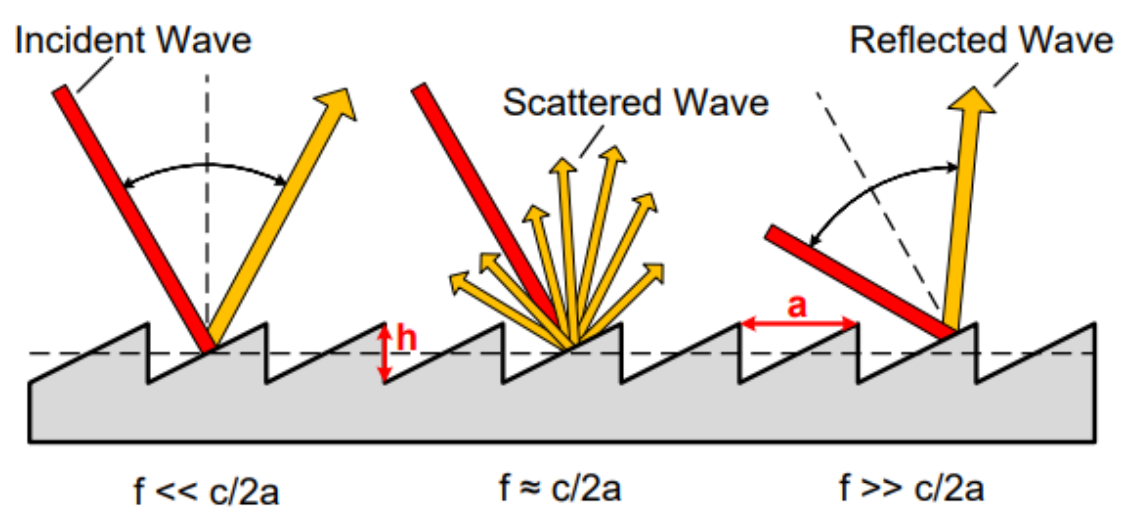
\includegraphics[width=0.6\textwidth]{figs/wave-reflexion.png}
    \captionsetup{justification=centering}
    \caption{Reflexiones en una superficie con irregularidades de altura h y largo a. \newline\textit{f} denota la frecuencia de la onda incidente y c su velocidad}
    \label{fig:refleccion}
\end{figure}

La \textbf{absorción} del sonido refiere al proceso en el cual una estructura u objeto es impactada por una onda de sonido determinada y, además de reflejar la onda, absorbe y transforma parte de su energía. Típicamente la energía absorbida es transformada en calor. Es un concepto crucial para controlar y manipular el sonido de forma predecible en determinados ambientes.

La efectividad de un material para reflejar un sonido está dado por su coeficiente de reflexión $R$ observado, inversamente, la efectividad en la absorción sobre el sonido se representa con su coeficiente de absorción $\alpha$, el cual varía de 0 (reflexión de onda absoluta) a 1 (absorción absoluta). Este coeficiente depende de varios factores del material, como su grosor, densidad, y la estructura de su superficie. Por ejemplo, la espuma plástica con la cual se elaboran los paneles acústicos que se utilizan para evitar la propagación del sonido es un material altamente poroso que permite que la onda de sonido traspase su superficie, para luego disipar la energía de la misma. Además no solo depende del material, sino que depende de la frecuencia del sonido y el ángulo con el cual la onda de sonido impacta con el material.

$R$ y $\alpha$ se calculan inversamente de la siguiente forma \cite{Moser}:

\begin{equation}
\alpha = 1 - (I_r/I_i)^2, \quad\quad R = 1 - \alpha
\end{equation}

Donde $I_r$ es la intensidad de la onda reflejada, e $I_i$ es la intensidad de la onda incidente o emitida

Además de la reflexión y la absorción, cuando el sonido impacta con un obstáculo hay un tercer fenómeno incidente, la transmisión del sonido a través del obstáculo (figura \ref{fig:interaccion}). Se trata de un concepto bastante natural para todas las personas, se puede observar al escuchar el sonido de otra habitación a través de la pared que la separa. Con seguridad el sonido transmitido tiene características más silenciosas y apagadas, especialmente en comparación con el sonido original, dado que las frecuencias más altas se aíslan más efectivamente que las más bajas \cite{Schroder}.

\begin{figure}[h!]
    \centering
    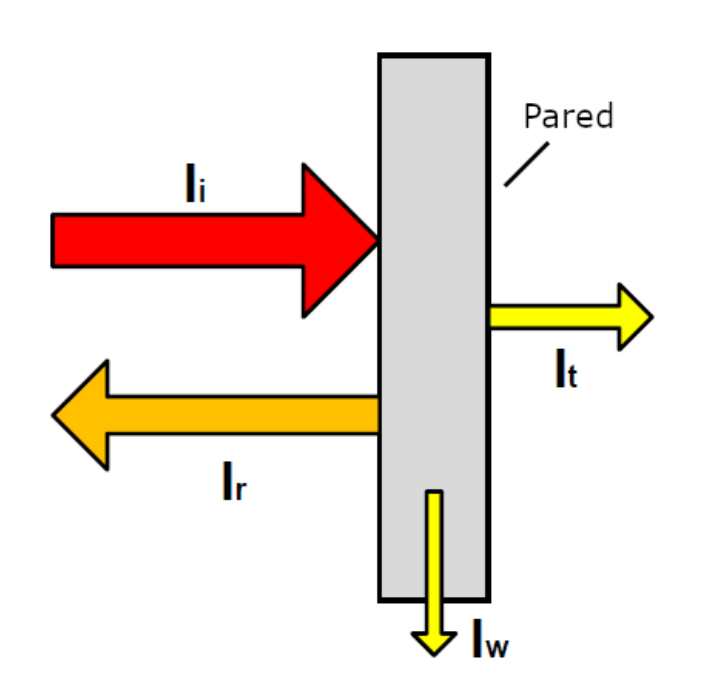
\includegraphics[width=0.4\textwidth]{figs/sound-interaction.png}
    \captionsetup{justification=centering}
    \caption{$I_i$ es la intensidad incidente del sonido, $I_r$ es la reflejada, $I_w$ es la absorbida y $I_t$ es la transmitida}
    \label{fig:interaccion}
\end{figure}

El índice de reducción de sonido es un indicador de qué tan bien un elemento constructivo, como una pared, techo o piso, puede atenuar el sonido. Se define por la relación entre la intensidad del sonido incidente $I_i$ en el elemento y la intensidad transmitida $I_t$. Matemáticamente, esto se representa como $R = -10log(I_i,I_t) $

La \textbf{refracción} del sonido, a diferencia de los conceptos anteriores, no está relacionada al impacto del sonido con un obstáculo. Este fenómeno cambia la dirección del sonido a causa de diferencias en la velocidad de propagación. Un ejemplo de esto se puede apreciar en la figura \ref{fig:refraccion}, donde la velocidad de un sonido transmitido sobre un medio denso es mayor que la velocidad de un medio menos denso. Esto causa que los frentes de onda marcados por los segmentos A-B y C-D ya no sean paralelos

\begin{figure}[h!]
    \centering
    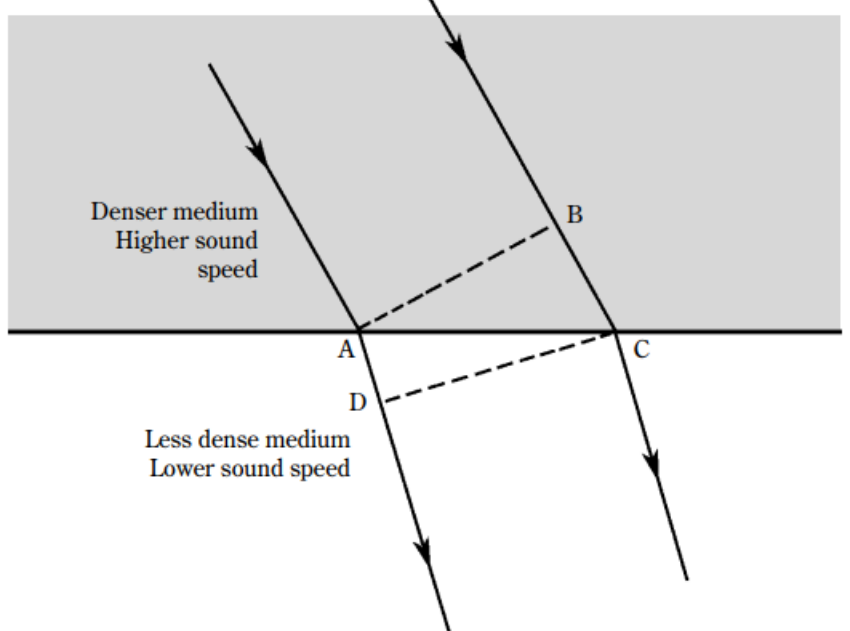
\includegraphics[width=0.7\textwidth]{figs/refraction.png}
    \captionsetup{justification=centering}
    \caption{Ejemplo de la trayectoria de una onda que atraviesa medios con distintas densidades. Extraído de \cite{Everest}}
    \label{fig:refraccion}
\end{figure}

Nuestra atmósfera no representa un medio uniforme para la propagación del sonido, es un sistema intensamente dinámico que desafía a los meteorólogos constantemente. Debido a esto, el comportamiento del sonido en la atmósfera se ve afectado por factores como la velocidad del aire, su temperatura, su composición, su densidad, entre otros. Sin embargo, en el contexto del proyecto el principal escenario de estudio son los espacios cerrados, donde si se puede considerar el aire como un medio uniforme ya que gran parte de estos factores se minimizan. El principal factor a considerar son las diferencias en la temperatura del aire causadas por artefactos como el aire acondicionado, ya que el sonido viaja más rápidamente en aire más caliente. De todas formas, no se consideró un factor relevante sobre la propagación del sonido en este proyecto.
\newpage % para que la siguiente figura quede bien
\begin{wrapfigure}{l}{0.5\textwidth}
    \centering
    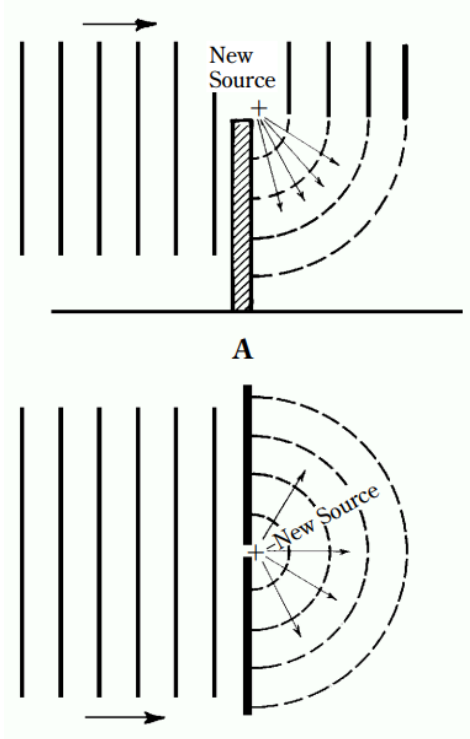
\includegraphics[width=0.4\textwidth]{figs/diffraction.png}
    \captionsetup{justification=centering}
    \caption{Ejemplo del fenomeno ocurriendo . Extraído de \cite{Everest}}
    \label{fig:difraccion}
\end{wrapfigure}

Por otro lado, el concepto de \textbf{difracción} describe el fenómeno donde la dirección del sonido es alterada no por cambios en el medio, sino por obstáculos presentados en su trayectoria. Un ejemplo básico de este fenómeno se puede reproducir fácilmente, reproduciendo música en una habitación de una casa se puede observar que esta es audible a lo largo de un pasillo o en otras habitaciones, “doblando” en cada esquina. En la figura \ref{fig:difraccion} se puede ver ejemplos de esto. Al impactar el sonido con una pared en el ejemplo A, se genera una nueva fuente virtual de sonido. De forma similar esto sucede en el ejemplo B, donde el sonido que atraviesa un agujero en la pared se convierte en una nueva fuente virtual, radiando el sonido omnidireccionalmente.

Existen más ejemplos y cada caso depende tanto del obstáculo como de la longitud de onda del sonido. Es importante destacar que la influencia de la difracción en espacios cerrados suele ser de un orden menor que la de las reflexiones. \newline \newline \newline \newline \newline % para que la siguiente figura quede bien

\subsection{Representación digital del sonido}

\subsubsection{Muestreo}

El primer paso en el almacenamiento digital del sonido es capturar la onda sonora. Esto se realiza típicamente utilizando un micrófono, los cuales son dispositivos electroacústicos que convierten la energía acústica en energía eléctrica. Todos los micrófonos poseen un “diafragma” o superficie móvil similar que es excitada por las variaciones en la presión generadas por la onda sonora. 

Mediante la utilización del micrófono se lleva a cabo el proceso de muestreo. En esta etapa, la señal analógica continua se convierte en una señal digital discreta. tomando instantáneas regulares o muestras de la amplitud de la señal analógica a intervalos fijos, lo que resulta en una serie de valores que aproximan la onda a lo largo de un tiempo dado. La frecuencia con la que se toman estas muestras se conoce como tasa de muestreo (o \textit{sample rate}), medida en hercios (Hz). Un sample rate común para audio de calidad CD estándar es de 44.1kHz, lo que significa que el audio se muestrea 44,100 veces por segundo. En la actualidad también es frecuente utilizar sample rates de 88.2kHz o 96kHz para grabaciones de alta fidelidad.

Sin embargo, es importante notar que tasas de muestreo más altas pueden efectivamente reducir la precisión en la conversión de audio a una señal digital.

Los micrófonos, en su diversidad, poseen características específicas que influyen directamente en el proceso de muestreo. Un aspecto crucial es la capacidad del micrófono para discriminar el sonido proveniente de diferentes direcciones, determinando así una salida multicanal, donde se registran y reproducen varias señales de audio de manera independiente.

En el contexto de los canales de audio, el sonido mono emplea un único canal, resultando en una reproducción idéntica tanto en el oído izquierdo como en el derecho. Por otro lado, el sonido estéreo, más prevalente en uso, utiliza dos canales. Esta configuración estéreo permite crear una percepción de profundidad y dirección en el sonido, mejorando la experiencia auditiva al proporcionar una sensación de espacio y ubicación del sonido más realista.

\subsubsection{Cuantización}

Tras el proceso de muestreo, se inicia el proceso de cuantización, en el cual cada valor muestreado de la señal de audio se debe representar mediante un valor numérico en el dominio digital.

Este proceso conlleva inherentemente un grado de aproximación, dado que el espectro continuo de la señal analógica necesita ser representado por un conjunto finito de valores digitales. La exactitud de esta representación depende de la profundidad de bits (bit depth), la cual determina la cantidad de bits asignados a cada valor muestreado. Por ejemplo, una profundidad de bits de 16, estándar en el audio de CD, permite 65,536 valores diferentes para cada muestra. 

Un mayor bit depth ofrece dos ventajas significativas. En primer lugar, posibilita una mayor cantidad de valores digitales posibles para cada muestra, lo que se traduce en una precisión incrementada. Además, estos valores no solo abarcan una precisión más elevada, sino también un rango dinámico más amplio, permitiendo representar digitalmente sonidos tanto sutiles como intensos.

No obstante, un mayor bit depth también implica ciertas desventajas. Por un lado, incrementa el requerimiento de espacio de almacenamiento; por ejemplo, un sonido almacenado con una profundidad de 32 bits ocupará el doble de espacio que el mismo sonido cuantizado con una profundidad de 16 bits. Además, al permitir la digitalización de sonidos con una mayor precisión, se pueden introducir variaciones mínimas en la señal, que podrían ser captadas del ambiente, generando así ruido, distorsión, y un aumento en la complejidad de procesamiento y manejo del archivo de audio.

\subsubsection{Codificación y compresión}

Las muestras cuantificadas se codifican en un formato digital, lo que resulta en una representación binaria del sonido. Estos datos binarios pueden comprimirse aún más para reducir el tamaño del archivo, utilizando métodos de compresión con pérdida (como MP3 o AAC) o sin pérdida (como FLAC o WAV).

\subsection{Respuesta al impulso}

Como fue explicado en detalle, cuando una fuente de sonido emite sonido en una habitación cerrada, las ondas sonoras que se propagan interactúan en los elementos constructivos de la habitación hasta que finalmente llegan al receptor. Por lo tanto, un evento auditivo percibido por un oyente no solo consiste en la onda inicial generada por la fuente, sino también en la respuesta de la habitación, que comprende reflexiones retrasadas y atenuadas. 

Si se emite una señal única e instantánea dentro de una escena (como por ejemplo un aplauso) y se utiliza un micrófono como receptor, se puede medir esta señal así como la respuesta de la escena al impulso emitido (por esto se define a esta medición como respuesta al impulso, o IR por sus siglas en inglés). Esta medición puede verse como la “huella acústica” de la escena o habitación en donde se emitió. Objetivamente, el IR refleja la energía que llega al receptor en cada instante de tiempo, esta energía puede expresarse en intensidad o con el cuadrado de la presión eficaz.

Se pueden identificar tres secciones de un IR causadas por distintas fuentes. Las secciones difieren en sus propiedades y también en la percepción y procesamiento por el oído humano

\begin{enumerate}
  \item Sonido Directo - Este primer impulso que llega, el más fuerte, es evaluado por el oído humano para localizar la fuente de sonido. El sonido directo se retrasa por la distancia entre la fuente y el receptor y solo se atenúa por el aire.
  \item Reflexiones Tempranas - Las primeras reflexiones de los elementos constructivos circundantes u otros obstáculos en la habitación llegan al oyente. Estas reflexiones (de bajo orden) se agregan al sonido directo inicial por el oído humano, lo que significa que no se pueden percibir por separado. La información sobre la fuente de sonido, como la posición, distancia, anchura de la fuente y volumen, están relacionadas principalmente con estas primeras reflexiones.
  \item Reverberación Tardía - Típicamente con un retraso de 50-80 ms al sonido directo, el número de reflexiones aumenta gradualmente y el oído humano ya no puede percibirlas como eventos individuales. Este campo de sonido difuso forma una reverberación tardía que es casi independiente de la posición del oyente, ya que el oído humano comienza a realizar una integración energética bastante aproximada durante un cierto intervalo de tiempo y campo angular. La reverberación es un atributo acústico muy importante y probablemente el más conspicuo de una habitación, ya que ciertas características, como el volumen y la forma de la habitación, están directamente asociadas con ella, lo que le da a la habitación su sonido muy individual.

\end{enumerate}

\begin{figure}
    \centering
    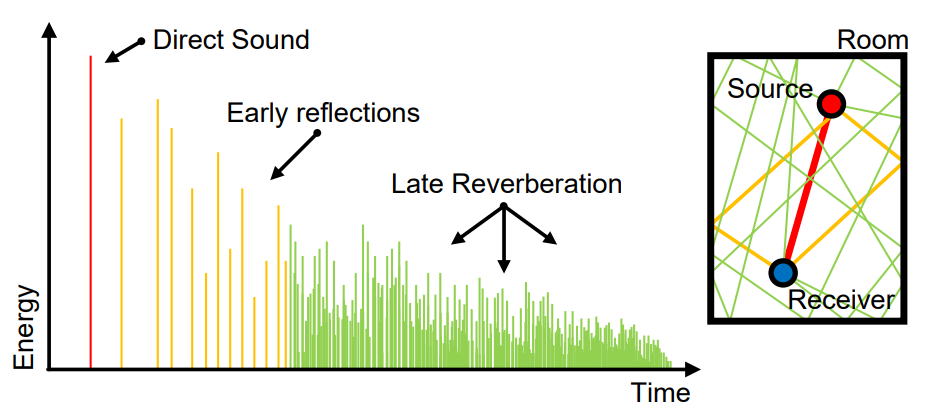
\includegraphics[width=0.7\textwidth]{figs/ir.png}
    \captionsetup{justification=centering}
    \caption{Ejemplo de un IR y sus secciones. Extraído de \cite{Ballou}}
    \label{fig:ir_example}
\end{figure}

Es de interés para este trabajo el IR ya que dado el mismo, es posible utilizarlo para simular como un sonido se escucharía si este fuera emitido por un emisor y recibido por un receptor posicionados dentro de la misma escena en la que se midió el IR, en sus posiciones originales. Este proceso se simula a través de una operación llamada convolución y se describe en mayor detalle posteriormente.

Es de interés para este trabajo el IR ya que dado el mismo, es posible utilizarlo para simular como un sonido se escucharía si este fuera emitido por un emisor y recibido por un receptor posicionados dentro de la misma escena en la que se midió el IR, en sus posiciones originales. Este proceso se simula a través de una operación llamada convolución y se describe en mayor detalle posteriormente. \colorbox{yellow}{Luego cuando tengamos escrita la parte de la implementacion se incluye una referencia aqui}

\subsubsection{Métodos de medición del IR}

Para grabar una respuesta al impulso fiel de un espacio, la fuente de sonido utilizada debe excitar el ambiente por igual en todas las frecuencias y en todas las direcciones.

Las primeras grabaciones de respuesta impulsiva se realizaban utilizando una fuente cuasi impulsiva, como el estallido de un globo \cite{Balloon}, un instrumento de percusión como un clapper (ver figura \ref{fig:clapper}) o un disparo \cite{York}. El uso de estas fuentes puede ser indeseable, ya que un disparo de un arma es inapropiado o prohibido en algunos contextos, y un instrumento de palmada es difícil de activar de forma remota y sin involucrar objetos reflectantes. Además, a causa las propiedades acústicas de cada objeto y/o experimento, se consideran que no ofrecen un verdadero impulso ya que no abarcan todas las frecuencias auditivas.

\begin{wrapfigure}{r}{0.5\textwidth}
    \centering
    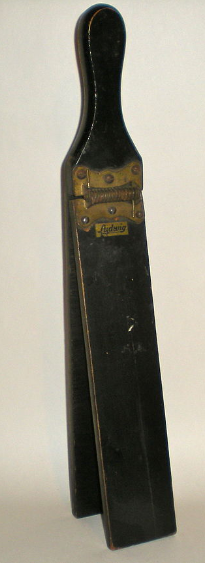
\includegraphics[width=0.2\textwidth]{figs/clapper.png}
    \captionsetup{justification=centering}
    \caption{Un \textit{clapper}, instrumento de percusión que consiste de dos tablas de maderas que se golpean para producir sonido.}
    \label{fig:clapper}
\end{wrapfigure}

Una onda sinusoidal “barrida” (de la traducción al inglés “sine sweep”) es una función sinusoidal que gradualmente cambia de frecuencia en el tiempo. Puede ser utilizada como una alternativa a los metrodos anteriores para emular la respuesta al impulso en todos los valores de frecuencia, proporcionando un barrido de amplitud constante a través de un rango de frecuencia adecuado que cubre típicamente el rango del oído humano (aproximadamente 20 Hz - 20 kHz). A diferencia de los métodos anteriores, el resultante es un audio extenso el cual se de-convoluye para obtener la respuesta al impulso y “remover” la onda sinusoidal de la grabación.

Es un método altamente popular dada su resultante exactitud. Sin embargo requiere un conjunto de equipos de grabación y reproducción, incluyendo un altavoz potente capaz de emitir en un amplio ancho de banda, lo cual resulta su principal desventaja en comparación a otros métodos, ya que los requisitos materiales y logísticos de esta técnica son significativos.

\subsection{Modelado del sonido como rayo}

Existen dos enfoques principales en el modelado acústico digital \cite{AcousticModeling}. El más preciso se basa en resolver numéricamente la ecuación de onda de sonido. Las técnicas que utilizan este enfoque se denominan basadas en ondas. El otro enfoque se basa en la acústica geométrica, en la cual se supone que el sonido actúa como rayos, dado que la dirección de la energía transmitida sigue la normal del frente de onda (ver figura \ref{fig:wavefront}). 

\begin{figure}
    \centering
    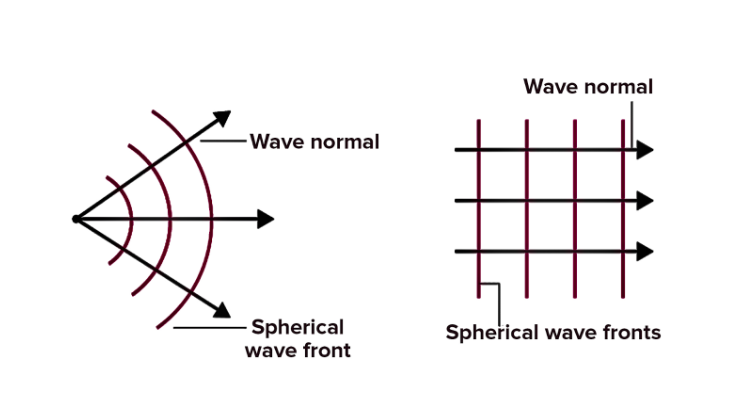
\includegraphics[width=0.7\textwidth]{figs/wavefront.png}
    \captionsetup{justification=centering}
    \caption{Dos tipos de frentes de onda y sus normales}
    \label{fig:wavefront}
\end{figure}

Sin embargo, utilizar esta simplificación significa una reducción en la precisión del modelado, ya que varios de los fenómenos basados en ondas, como la difracción y la refracción, están ausentes en estos métodos (en contraste a los métodos basados en ondas, ya que estos modelan los fenómenos de manera inherente). Es relevante mencionar que la difracción y la refracción se ven más presentes a bajas frecuencias, causando que el trazado no sea tan impreciso a altas frecuencias.

Otro factor que afecta la precisión de la simulación en la acústica geométrica es su capacidad limitada para encontrar todas las trayectorias de reflexión especular. Los métodos basados en ondas garantizan encontrar todas ellas, mientras que el trazado de rayos solo muestrean el espacio de trayectorias y modelan cierto subconjunto de todos los posibles caminos del sonido. Con una cantidad infinita de rayos, los resultados son los mismos entre los métodos, pero cuanto menos rayos se usen, es más probable que se pierdan trayectorias de reflexión.

En cuanto a los métodos basados en ondas, estos típicamente mantienen un conjunto constante de demandas computacionales para toda etapa de la simulación, ya que normalmente utilizan un número constante de elementos. Desafortunadamente, los costos computacionales son altos, ya que en muchos casos se debe resolver un enorme sistema lineal de ecuaciones. El tamaño del sistema depende de la frecuencia ya que debe haber un cierto número de elementos por longitud de onda. Esto implica que estos métodos son más adecuados para bajas frecuencias.

Claramente, existen ventajas y desventajas inherentes a cada enfoque, y cabe destacar que a lo largo del tiempo han surgido métodos híbridos que buscan combinar los aspectos más beneficiosos de ambos. Sin embargo, para los propósitos de este trabajo, se ha decidido optar por representar el sonido mediante el enfoque de trazado de rayos. Esta decisión se fundamenta principalmente en las  desventajas del método basado en ondas, en particular su complejidad.

\section{Fundamentos de la computación gráfica}

\subsection{Rasterización}

La técnica de rasterización es ampliamente utilizada en el campo de la computación gráfica para mostrar objetos tridimensionales en una superficie bidimensional. Funciona a partir de la representación digital de los objetos tridimensionales, estos se crean a partir de una malla de polígonos virtuales, generalmente triángulos, que forman el modelo tridimensional de los objetos. Cada polígono lleva asociada una gran cantidad de información, como su posición en el espacio, su color, textura y principalmente su vector normal, el cual indica la orientación de la superficie del objeto.

Una vez que se ha generado la malla de polígonos de la escena, un rasterizador procede a analizarla de manera eficiente mediante un algoritmo que gira a través de los polígonos para identificar aquellos píxeles en la pantalla que corresponden a los polígonos seleccionados. Este paso es crucial para determinar qué partes de los polígonos son visibles al observador. A continuación, se asigna un color a estos píxeles basándose en las propiedades específicas del polígono correspondiente, como su textura y color inherente, así como la forma en que la luz interactúa con él.

Versiones modernas de un rasterizador pueden incluir procesamiento adicional para determinar el color de los píxeles, como la iluminación dinámica de la escena, y otros efectos visuales avanzados.

\subsection{Ray Tracing}

El trazado de rayos, o ray tracing como es conocido en inglés, es una técnica inspirada en el comportamiento físico de la luz utilizada principalmente en la computación gráfica para la síntesis de imágenes de una escena tridimensional \cite{Raytracing}. En comparación a la rasterización se podría decir que se trata de un proceso inverso. En este método se simula la luz como una serie de rayos originarios desde la posición de un observador son emitidos en una dirección “a través” de un plano de imagen. El plano representa la pantalla, formada por una matriz de píxeles donde a cada píxel le corresponde un rayo emitido. El rayo procede a interactuar con la escena tridimensional de variadas formas para determinar el color que este debe de tener.

\begin{figure}[h!]
    \centering
    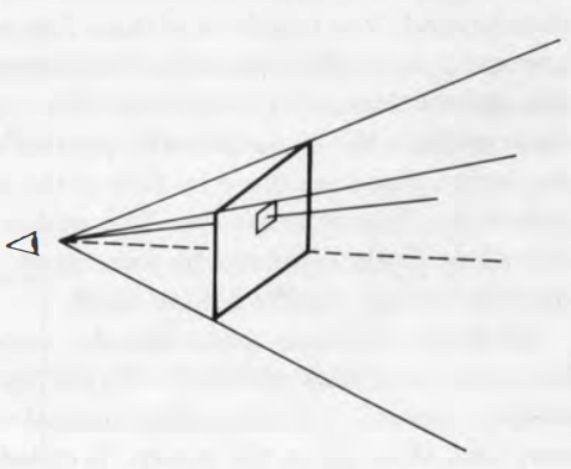
\includegraphics[width=0.7\textwidth]{figs/simplified-raytracer.png}
    \captionsetup{justification=centering}
    \caption{Elementos básicos de un raytracer, un punto de emisión (ojo del observador), un plano que representa la imagen y direcciona los rayos a través de sus “píxeles”}
    \label{fig:raytracer}
\end{figure}

\colorbox{yellow}{Work in progress, se continua escribiendo sobre el proceso de cálculo de la trayectoria de la luz}\newline
\colorbox{yellow}{ y su interacción con objetos virtuales.}

\subsection{Path Tracing}

\subsection{Tecnologías Asociadas al Trazado de Rayos}

\section{Simulación y Auralización}
%%%%%%%%%%%%%%%%%%%%%%%%%%%%%%%%%%%%%%%%%%%%%%%%%%%%%%%%%%%%%%%%%%%%%%%%%%%%%%%%%%%%%%%%%%%%%%%%

% parte central
\chapter{Parte Central}
La parte central del trabajo refiere a lo que es producción propia o aporte del
proyecto de grado, incluyendo las decisiones tomadas. Por ejemplo, puede incluir
los requerimientos, el análisis y el diseño de la solución. Si el proyecto tiene una
implementación, debe describirse en términos de decisiones tomadas en ese sentido.
Los detalles de programación se dejan para los anexos.

Se pueden incluir figuras y tablas en el documento, las mismas deben estar referenciadas en el texto. Por ejemplo, la Figura~\ref{fig:logos} muestra los logos de Facultad de Ingeniería y de la Universidad de la República, mientras que la Tabla~\ref{table:datos} tiene números aleatorios.

\begin{figure}[h!]
    \centering
    
\includegraphics[width=\textwidth]{figs/logo-udelar-fing.png}
    \caption{Logos de FIng y UdelaR}
    \label{fig:logos}
\end{figure}

\begin{table}[h!]
\centering
\begin{tabular}{| c | c | c | c |} 
 \hline
 Col1 & Col2 & Col2 & Col3 \\  
 \hline
 1 & 970 & 67 & 941 \\ 
 2 & 668 & 845 & 141 \\
 3 & 800 & 383 & 464 \\
 4 & 143 & 683 & 502 \\
 \hline
\end{tabular}
\caption{Tabla con datos}
\label{table:datos}
\end{table}

%%%%%%%%%%%%%%%%%%%%%%%%%%%%%%%%%%%%%%%%%%%%%%%%%%%%%%%%%%%%%%%%%%%%%%%%%%%%%%%%%%%%%%%%%%%%%%%%

% Primeros pasos
\chapter{Primeros pasos}

\section{Setup}

El proyecto inicialmente fue pensado para basarse en el proyecto de grado de Camilo Satut y utilizar el poder de procesamiento de datos de las tarjetas de video para lograr realizar más cálculos en paralelo y así obtener una mejor calidad de audio, junto con otros beneficios. La gran mayoría del tiempo invertido en las primeras semanas fue destinado a entender la implementación de Camilo y discutir donde y como se deberían implementar dichas mejoras.

A partir de estas reuniones se construyó un backlog de requerimientos, ideas y mejoras posibles para ir priorizando e implementando. 

Se estableció un plan de trabajo estilo scrum donde utilizamos sprints con una duración de 2 semanas y al final del sprint se tenía una reunión con el tutor para reportar los avances y discutir posibles soluciones. 

El priemr sprint fue totalmente dedicado a la investigación de Optix y multiples biblioteca de audio. En este sprint el entregable fue poder realizar un render sobre la tarjeta de video y luego de checkear distintas bibliotecas de audio se decidió continuar con 



%%%%%%%%%%%%%%%%%%%%%%%%%%%%%%%%%%%%%%%%%%%%%%%%%%%%%%%%%%%%%%%%%%%%%%%%%%%%%%%%%%%%%%%%%%%%%%%%

%%%%%%%%%%%%%%%%%%%%%%%%%%%%%%%%%%%%%%%%%%%%%%%%%%%%%%%%%%%%%%%%%%%%%%%%%%%%%%%%%%%%%%%%%%%%%%%%

% experimentación
\chapter{Experimentación}
Puede ser necesario incluir un capítulo de Experimentación, incluyendo las pruebas realizadas (casos de prueba) y los resultados obtenidos con su respectivo análisis, que puede incluir comparaciones. 

%%%%%%%%%%%%%%%%%%%%%%%%%%%%%%%%%%%%%%%%%%%%%%%%%%%%%%%%%%%%%%%%%%%%%%%%%%%%%%%%%%%%%%%%%%%%%%%%

%conclusiones
\chapter{Conclusiones y Trabajo Futuro}

En este capítulo se evalúan los resultados alcanzados y
dificultades encontradas, se establece lo que se planteó hacer y lo que se hizo
realmente, cuales fueron los aportes, se muestran posibles extensiones al trabajo, se
realiza una autocrítica de lo que se hizo y lo que faltó (por problemas de tiempo,
recursos, cómo se puede continuar, qué cosas hacer, prioridades, etc.) y se incluye
información sobre la gestión del proyecto, si aplica

%%%%%%%%%%%%%%%%%%%%%%%%%%%%%%%%%%%%%%%%%%%%%%%%%%%%%%%%%%%%%%%%%%%%%%%%%%%%%%%%%%%%%%%%%%%%%%%%
% Parte final
%%%%%%%%%%%%%%%%%%%%%%%%%%%%%%%%%%%%%%%%%%%%%%%%%%%%%%%%%%%%%%%%%%%%%%%%%%%%%%%%%%%%%%%%%%%%%%%%

{ % inicio backmatter

\backmatter % no numerar capítulos 

% referencias bibliográficas

\newpage
\bibliographystyle{apacite}
\bibliography{referencias}

} % fin backmatter

%%%%%%%%%%%%%%%%%%%%%%%%%%%%%%%%%%%%%%%%%%%%%%%%%%%%%%%%%%%%%%%%%%%%%%%%%%%%%%%%%%%%%%%%%%%%%%%%

% anexos

\begin{appendix}

\chapter{Anexo 1}

Los anexos contienen información adjunta al proyecto pero que no es fundamental
para entender el trabajo. Por ejemplo, determinado material de los antecedentes o la
implementación, que en el cuerpo principal del informe se encuentre resumido, aquí
puede presentarse de forma completa. En caso de proyectos de desarrollo de
software, se debería incluir un manual de usuario.

\section{Sección del Anexo}

Los anexos pueden tener secciones.

\end{appendix}


%%%%%%%%%%%%%%%%%%%%%%%%%%%%%%%%%%%%%%%%%%%%%%%%%%%%%%%%%%%%%%%%%%%%%%%%%%%%%%%%%%%%%%%%%%%%%%%%

\end{document}
